\chapter{Pruebas Experimentales} % Título del capítulo
\label{Chapter5}
\lhead{Capítulo 5. \emph{Pruebas Experimentales}}

% NOTA: Las tablas de este capítulo se generan automáticamente desde los datos
% del experimento con:
%   python scripts/generate_experiment_figures.py --update-book
% que las escribe en docs/libro/Tables/*.tex y copia las figuras a
% docs/libro/Figures/capitulo5/. Al regenerar el experimento, el capítulo se
% actualiza sin ediciones manuales (salvo la discusión).

Este capítulo presenta los resultados de la evaluación experimental del framework sobre una muestra representativa de ortopantomografías, siguiendo el diseño descrito en la Sección~\ref{sec:diseno_experimental}.

\section{Configuración experimental}

El experimento procesó una muestra aleatoria estratificada de 83 imágenes (nivel de confianza del 95\%, margen de error $\pm 10\%$, Ecuación~\ref{eq:cochran}) de la población de 598 ortopantomografías. Cada imagen fue sometida a una degradación controlada aleatoria (Sección~\ref{sec:degradacion}) y procesada por el framework completo con la configuración canónica de SMPSO (Tabla~\ref{tab:config_smpso}). La Tabla~\ref{tab:resumen_ejecucion} resume la ejecución.

\begin{table}[H]
\centering
\caption[Resumen de la ejecución experimental]{Resumen de la ejecución experimental.}
\label{tab:resumen_ejecucion}
\begin{tabular}{ll}
\hline
\textbf{Parámetro} & \textbf{Valor} \\
\hline
Imágenes procesadas & 83 de 83 muestreadas \\
Partículas / iteraciones SMPSO & 100 / 100 \\
Semilla & 42 \\
Tiempo total (5 procesos en paralelo) & 6.8 h \\
Tiempo promedio por imagen & 24.2 $\pm$ 3.9 min \\
Tamaño promedio del Frente de Pareto & 100.0 $\pm$ 0.1 \\
Degradaciones aplicadas & Bajo contraste: 24, Sobreexposición: 16, Subexposición: 15, Histograma sesgado: 14, Bajo contraste local: 14 \\
\hline
\end{tabular}
\end{table}

\section{Resultados de la etapa de optimización}

\subsection{Frentes de Pareto obtenidos}

SMPSO alcanzó en todas las imágenes el tamaño máximo del archivo externo ($100.0 \pm 0.1$ soluciones no dominadas). Este dato debe interpretarse con precisión: la saturación indica que el algoritmo produjo soluciones no dominadas en cantidad suficiente para llenar el archivo, pero no constituye por sí misma evidencia de convergencia; implica, además, que la poda por distancia de apiñamiento estuvo activa, de modo que el tamaño del archivo ---y no la capacidad de búsqueda--- es el límite efectivo de la cobertura del frente. Ambas cuestiones (convergencia del proceso y efecto del tamaño del archivo sobre la cobertura) se examinan empíricamente en la Sección~\ref{sec:convergencia}.

La Figura~\ref{fig:pareto_ejemplo} muestra el Frente de Pareto de una imagen representativa, junto con las selecciones de los ocho métodos MCDM y la solución de consenso. Las proyecciones bidimensionales evidencian el conflicto entre los objetivos: las soluciones de mayor entropía (realce agresivo) sacrifican SSIM (fidelidad estructural), mientras que el VIF crece junto con la entropía en este régimen y alcanza sus máximos en las configuraciones de mayor realce que aún no destruyen información. Los métodos compensatorios seleccionan sistemáticamente en la región de alto VIF del frente, mientras que Bellman-Zadeh elige en la zona central equilibrada.

\begin{figure}[H]
    \centering
    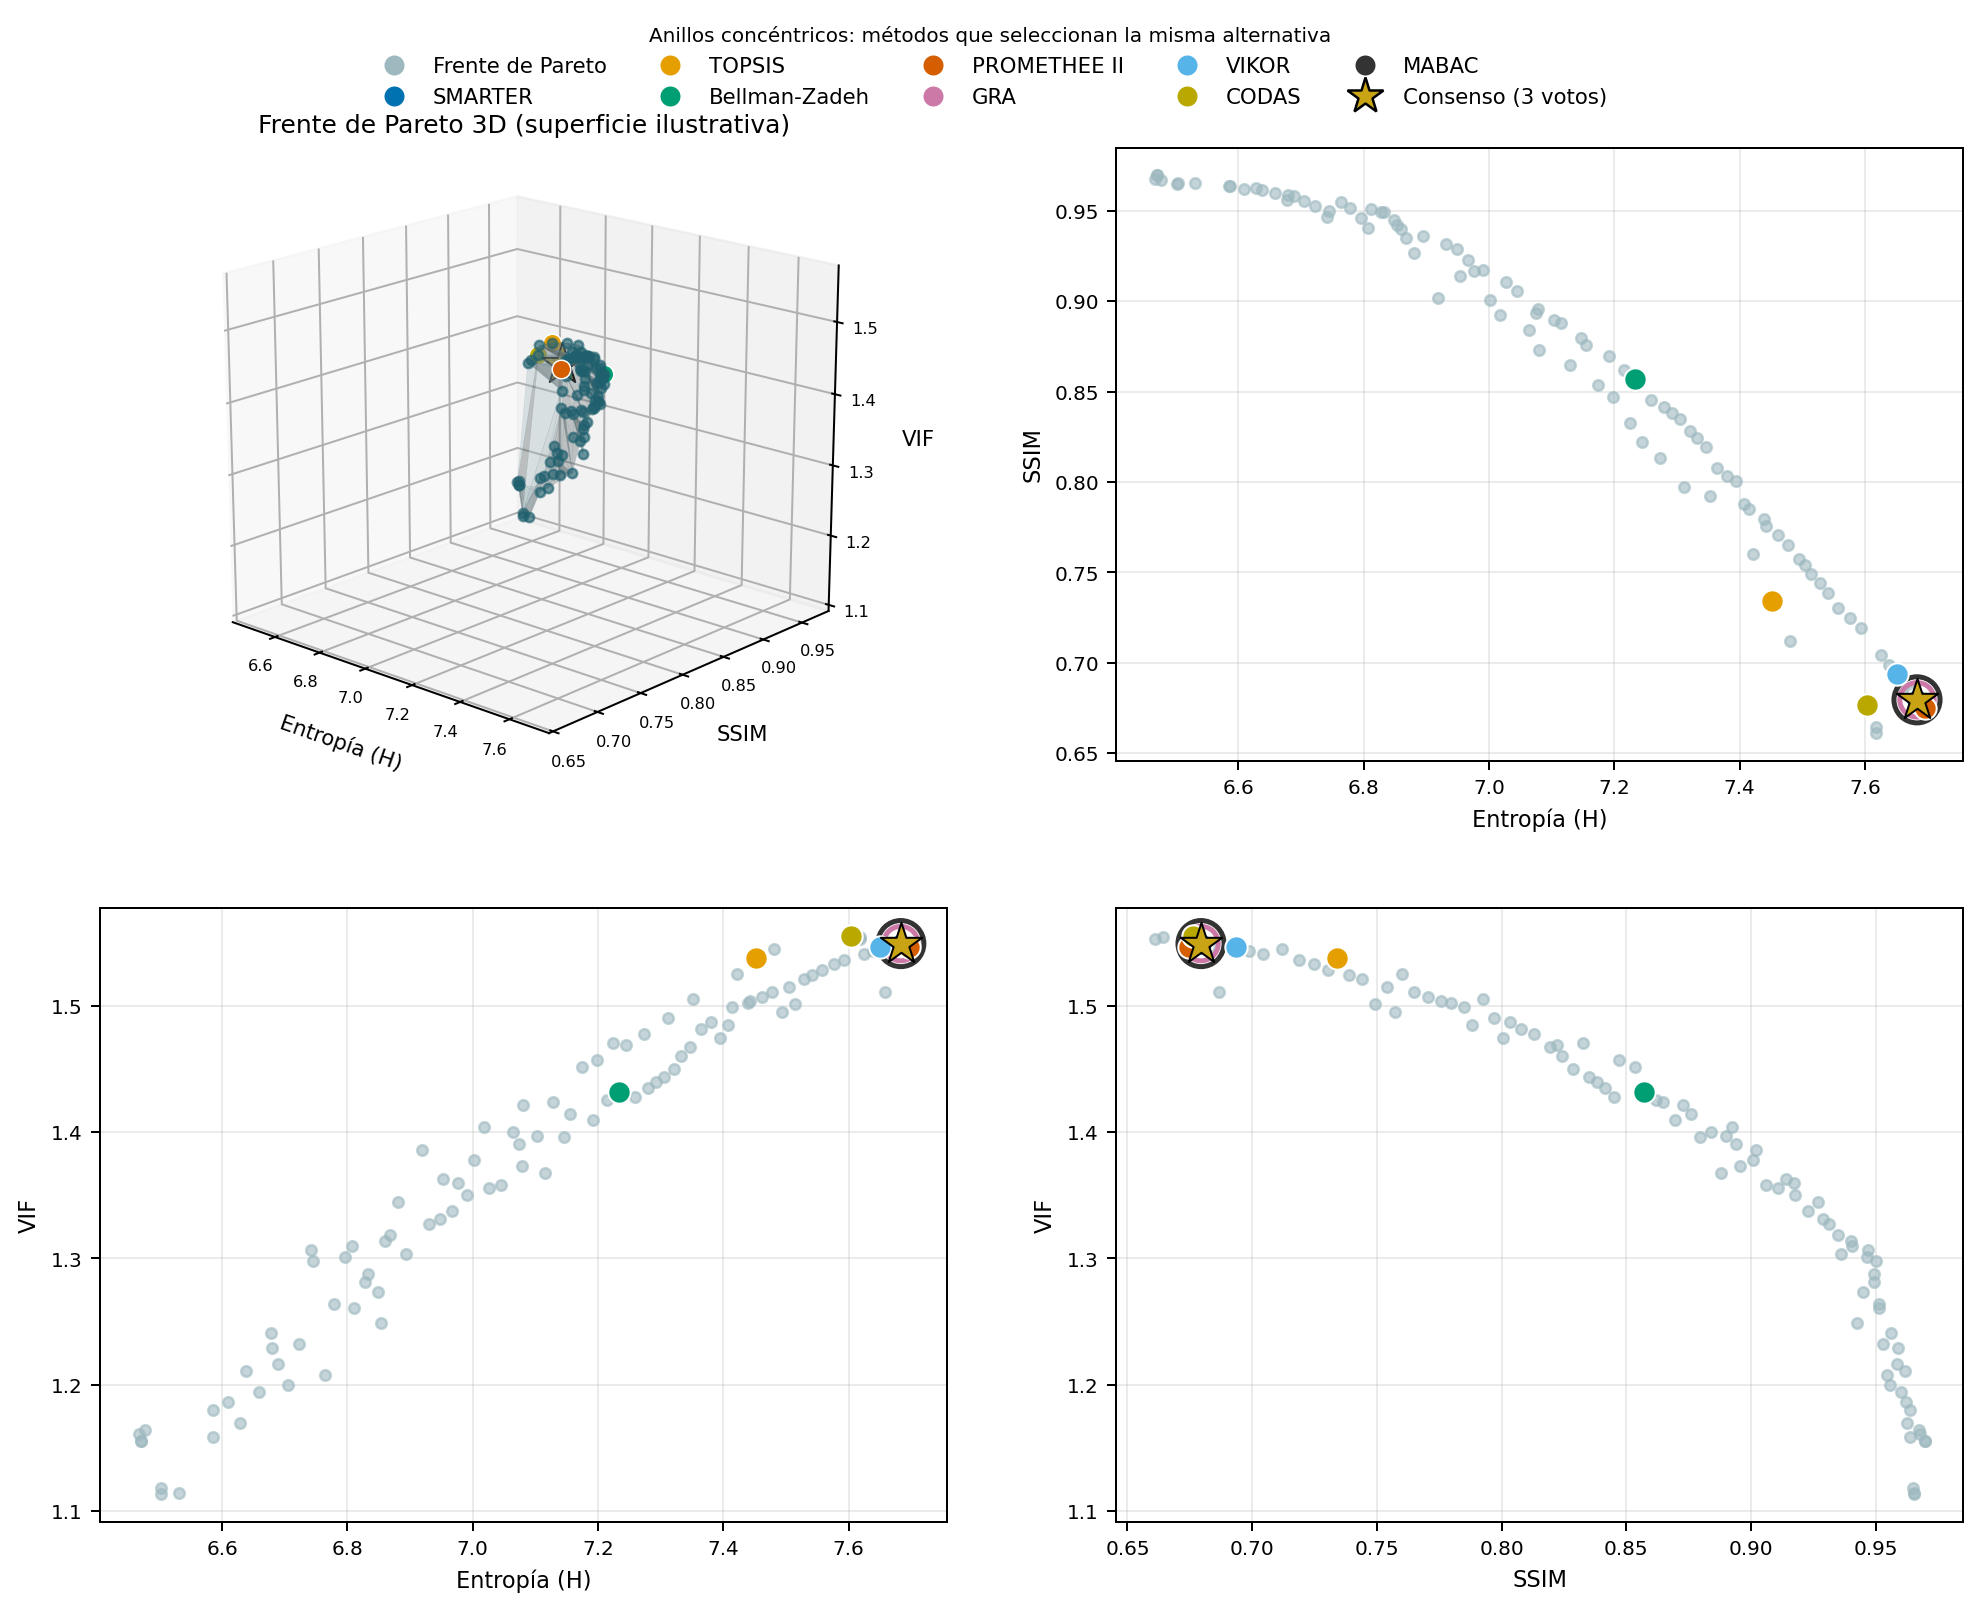
\includegraphics[width=0.9\textwidth]{./Figures/capitulo5/pareto_low_contrast}
    \caption[Frente de Pareto de una imagen representativa]{Frente de Pareto (entropía, SSIM, VIF) de una imagen representativa degradada con bajo contraste global: panel 3D con superficie ilustrativa obtenida por triangulación de las soluciones no dominadas, y proyecciones bidimensionales de cada par de objetivos. Cada círculo de color indica la selección de un método MCDM; los anillos concéntricos señalan métodos que seleccionaron la misma alternativa, y la estrella dorada la solución de consenso. La superficie es una ayuda visual: el frente es un conjunto discreto de puntos y la interpolación no implica continuidad.}
    \label{fig:pareto_ejemplo}
\end{figure}

\subsection{Métricas de las soluciones seleccionadas}

La Tabla~\ref{tab:metricas_compromiso} presenta las estadísticas de las métricas de calidad de la solución seleccionada por consenso sobre las 83 imágenes. Es destacable que el VIF medio de las soluciones seleccionadas supera la unidad ($1.1875 \pm 0.2621$): la imagen realzada contiene, en promedio, \textit{más} información visual extraíble que la imagen degradada que ingresó al framework, comportamiento que el VIF captura y que ninguna métrica acotada en $[0,1]$ como el SSIM podría expresar.

\begin{table}[H]
\centering
\caption[Métricas de calidad de la solución seleccionada]{Estadísticas de las métricas de calidad de la solución seleccionada por consenso (media $\pm$ desviación estándar, intervalo de confianza del 95\% y rango).}
\label{tab:metricas_compromiso}
\begin{tabular}{lccc}
\hline
\textbf{Métrica} & \textbf{Media $\pm$ DE} & \textbf{IC 95\%} & \textbf{Rango} \\
\hline
Entropía (H) & 7.1494 $\pm$ 1.2095 & [6.8853, 7.4135] & [3.1353, 7.8548] \\
SSIM & 0.7836 $\pm$ 0.1610 & [0.7484, 0.8187] & [0.2696, 0.9652] \\
VIF & 1.1875 $\pm$ 0.2621 & [1.1302, 1.2447] & [0.9569, 1.9067] \\
\hline
\end{tabular}
\end{table}

\subsection{Parámetros CLAHE seleccionados}

La Tabla~\ref{tab:parametros_clahe} y la Figura~\ref{fig:parametros_clahe} describen la distribución de los parámetros CLAHE de las soluciones seleccionadas. Los parámetros se concentran marcadamente en la región de regiones contextuales pequeñas ($R_x = 4.9 \pm 5.1$, $R_y = 3.7 \pm 3.2$, con moda $2$ en ambos casos), es decir, en un realce de carácter cuasi-global. Este resultado es coherente con la naturaleza de las degradaciones aplicadas, que son predominantemente globales (compresión del rango dinámico, transformaciones gamma, sesgo del histograma): el proceso de optimización descubre que un particionamiento fino de la imagen no aporta beneficio cuando el deterioro no es local, y que en cambio introduce artefactos que penalizan el SSIM y el VIF. El límite de recorte se distribuye ampliamente ($C = 2.06 \pm 1.11$) a lo largo de todo el dominio $[1, 4]$, reflejando que la intensidad del realce necesaria sí depende fuertemente de la severidad de la degradación de cada imagen.

\begin{table}[H]
\centering
\caption[Parámetros CLAHE de las soluciones seleccionadas]{Distribución de los parámetros CLAHE de las soluciones seleccionadas por consenso.}
\label{tab:parametros_clahe}
\begin{tabular}{lcccc}
\hline
\textbf{Parámetro} & \textbf{Media} & \textbf{DE} & \textbf{Moda} & \textbf{Rango} \\
\hline
$R_x$ & 4.9 & 5.1 & 2.0 & [2.0, 39.0] \\
$R_y$ & 3.7 & 3.2 & 2.0 & [2.0, 22.0] \\
$C$ & 2.057 & 1.106 & 1.000 & [1.000, 4.000] \\
\hline
\end{tabular}
\end{table}

\begin{figure}[H]
    \centering
    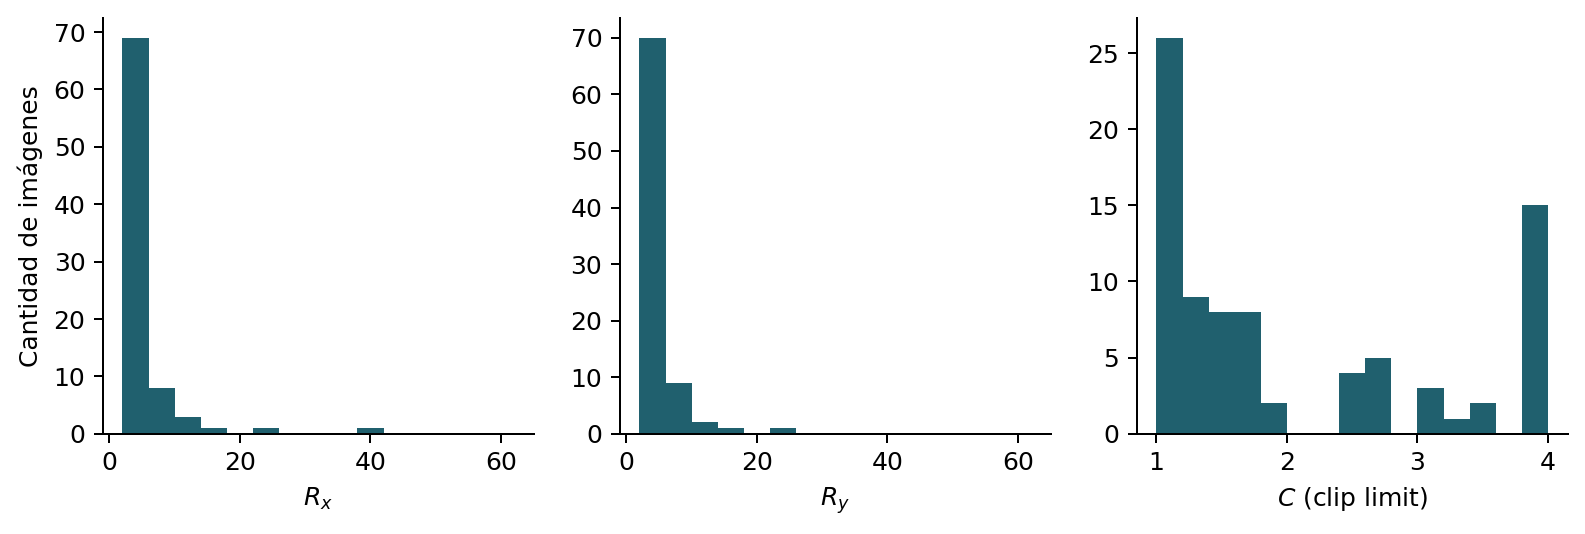
\includegraphics[width=\textwidth]{./Figures/capitulo5/parametros_clahe}
    \caption[Distribución de los parámetros CLAHE seleccionados]{Histogramas de los parámetros CLAHE ($R_x$, $R_y$, $C$) de las soluciones seleccionadas por consenso sobre la muestra.}
    \label{fig:parametros_clahe}
\end{figure}

\section{Validación contra la imagen original}
\label{sec:validacion_original}

La degradación controlada permite medir la recuperación de calidad respecto a la imagen original (\textit{ground truth}), un análisis imposible en escenarios sin referencia. La Tabla~\ref{tab:validacion} resume las métricas de la imagen degradada (entrada del framework) y de la imagen mejorada (salida) calculadas contra la original.

\begin{table}[H]
\centering
\caption[Recuperación de calidad respecto a la imagen original]{Recuperación de calidad respecto a la imagen original: métricas de la imagen degradada (entrada) y de la imagen mejorada seleccionada por consenso (salida), ambas contra la original.}
\label{tab:validacion}
\begin{tabular}{lccc}
\hline
\textbf{Métrica vs. original} & \textbf{Degradada} & \textbf{Mejorada} & \textbf{Recuperación} \\
\hline
SSIM & 0.7208 $\pm$ 0.2484 & 0.7936 $\pm$ 0.1900 & +0.0728 \\
VIF & 0.6823 $\pm$ 0.2063 & 0.9499 $\pm$ 0.1708 & +0.2676 \\
\hline
\end{tabular}
\end{table}

El resultado es inequívoco: \textbf{las 83 imágenes de la muestra (100\%) recuperaron fidelidad de información visual} respecto a la original, con una ganancia media de VIF de $+0.2676$ (de $0.6823$ a $0.9499$). La diferencia es estadísticamente significativa según la prueba de rangos con signo de Wilcoxon ($W = 0$, $p < 10^{-14}$), y el valor $W = 0$ indica que no existió una sola imagen en la que el realce empeorara el VIF. En términos de similitud estructural, 68 de las 83 imágenes (81.9\%) mejoraron su SSIM respecto a la original, con una ganancia media de $+0.0728$ ($W = 391$, $p < 10^{-9}$). La menor tasa de mejora del SSIM frente al VIF es esperable y consistente con el planteamiento del Capítulo~\ref{Chapter2}: el SSIM penaliza toda alteración estructural, incluso aquella que restituye contraste diagnóstico, mientras que el VIF valora la información visual efectivamente recuperada.

La Figura~\ref{fig:recuperacion_vif} presenta la recuperación imagen por imagen: cada punto por encima de la diagonal corresponde a una imagen cuya versión mejorada es más fiel a la original que la versión degradada que ingresó al framework. La Figura~\ref{fig:recuperacion_por_degradacion} desagrega la recuperación por tipo de degradación, evidenciando una fuerte dependencia del tipo de deterioro: el framework recupera de forma sobresaliente el bajo contraste global ($+0.497 \pm 0.078$), seguido del histograma sesgado ($+0.227 \pm 0.106$), la sobreexposición ($+0.178 \pm 0.058$), la subexposición ($+0.165 \pm 0.077$) y, en último lugar, el bajo contraste local ($+0.128 \pm 0.032$). Este ordenamiento es interpretable: CLAHE es, en esencia, un redistribuidor del histograma, por lo que su capacidad de recuperación es máxima cuando la degradación consiste precisamente en una compresión del rango dinámico, y mínima cuando la información se ha perdido por suavizado espacial (bajo contraste local), donde el detalle destruido no puede restituirse por reasignación de intensidades.

\begin{figure}[H]
    \centering
    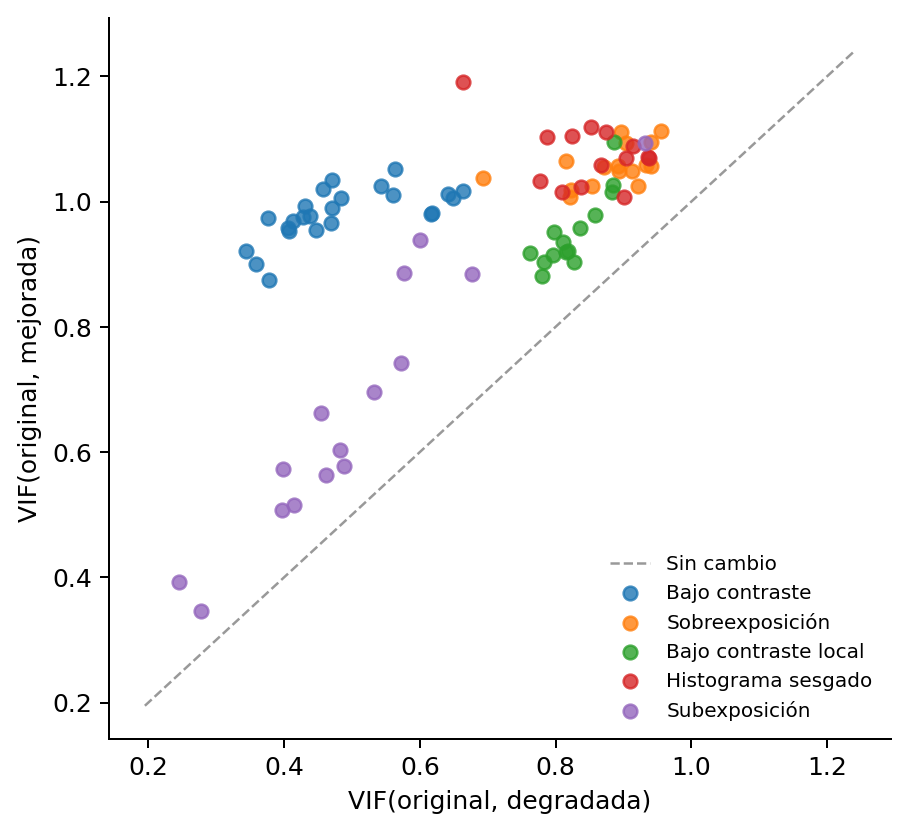
\includegraphics[width=0.62\textwidth]{./Figures/capitulo5/recuperacion_vif}
    \caption[Recuperación de VIF respecto a la original]{VIF de la imagen mejorada vs. VIF de la imagen degradada, ambos calculados contra la original. Los puntos sobre la diagonal indican recuperación de información visual.}
    \label{fig:recuperacion_vif}
\end{figure}

\begin{figure}[H]
    \centering
    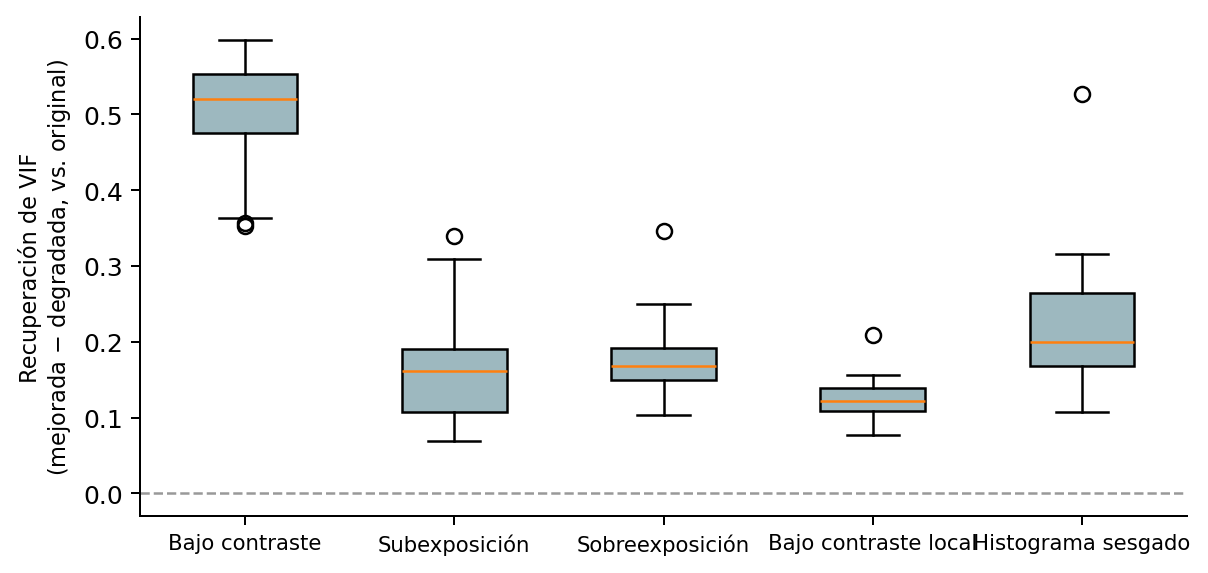
\includegraphics[width=0.85\textwidth]{./Figures/capitulo5/recuperacion_por_degradacion}
    \caption[Recuperación de VIF por tipo de degradación]{Distribución de la recuperación de VIF según el tipo de degradación aplicada.}
    \label{fig:recuperacion_por_degradacion}
\end{figure}

La Figura~\ref{fig:trios} ilustra el resultado visual del framework sobre imágenes representativas de distintos tipos de degradación.

\begin{figure}[H]
    \centering
    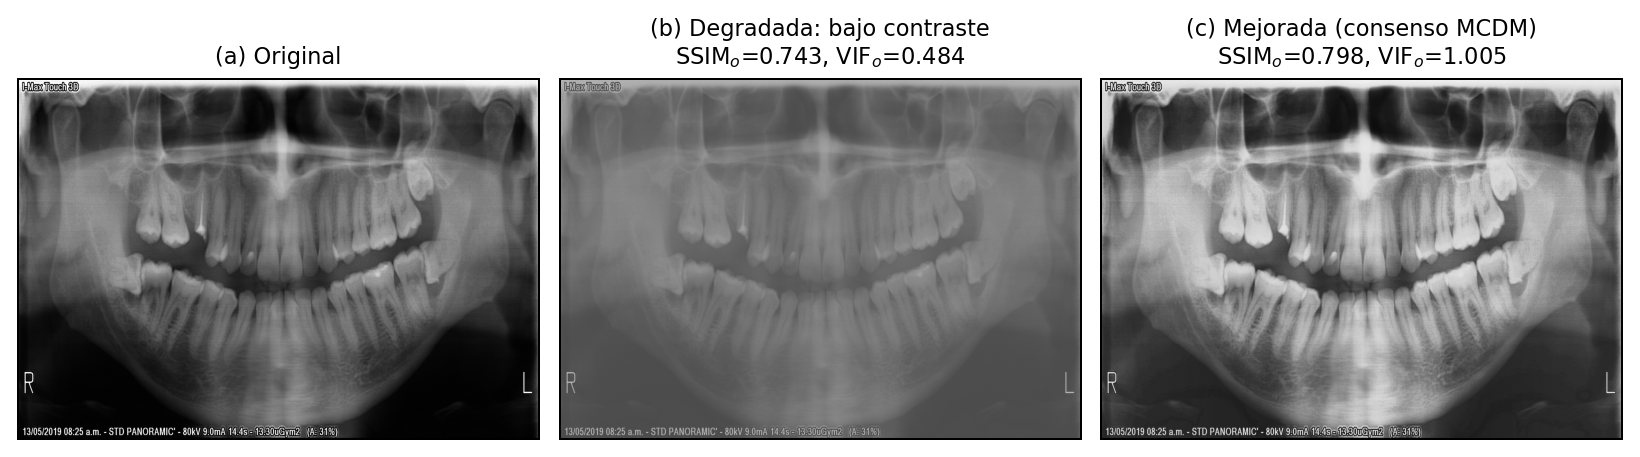
\includegraphics[width=\textwidth]{./Figures/capitulo5/trio_low_contrast}\\[2mm]
    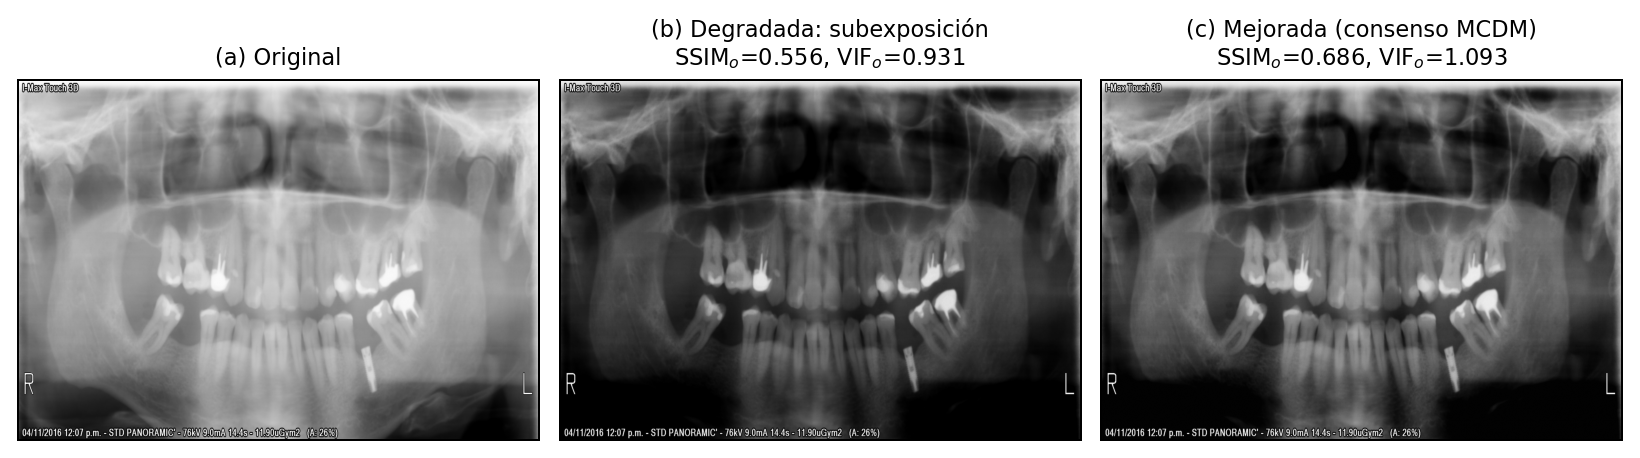
\includegraphics[width=\textwidth]{./Figures/capitulo5/trio_underexposure}\\[2mm]
    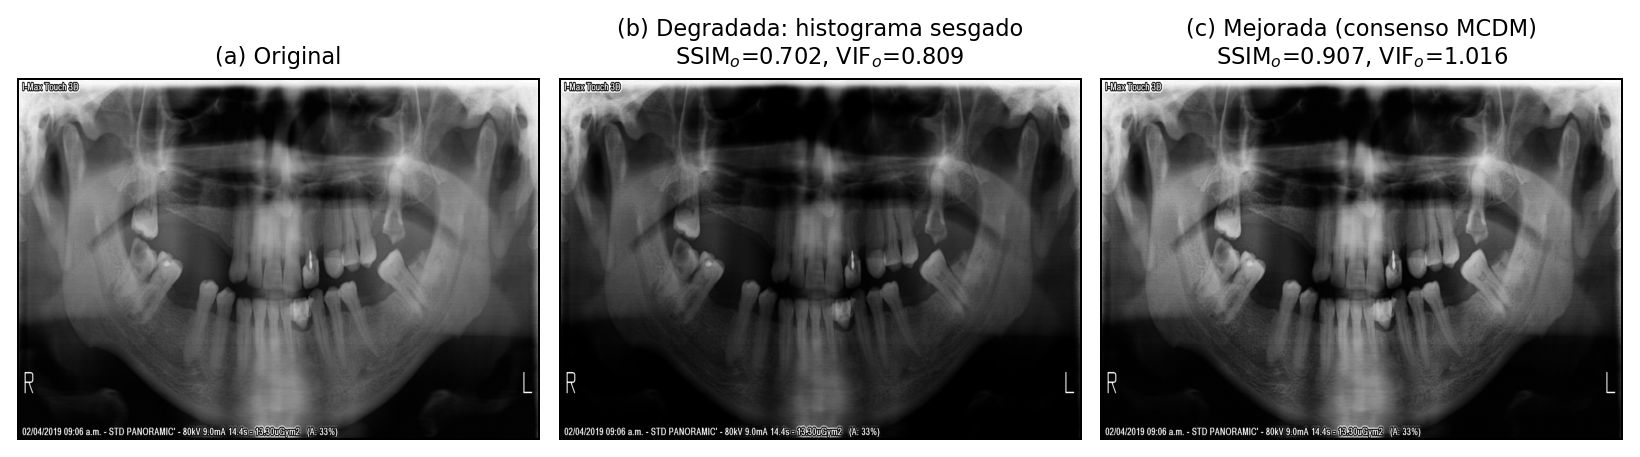
\includegraphics[width=\textwidth]{./Figures/capitulo5/trio_skewed_histogram}
    \caption[Resultados visuales sobre imágenes representativas]{Resultados visuales del framework sobre imágenes representativas (recuperación de VIF mediana de su grupo): bajo contraste global (arriba), subexposición (centro) e histograma sesgado (abajo). Cada fila muestra la imagen original, la degradada (entrada) y la mejorada seleccionada por consenso (salida), con sus métricas contra la original.}
    \label{fig:trios}
\end{figure}

\section{Resultados de la etapa de decisión}

\subsection{Concordancia entre métodos}

La Tabla~\ref{tab:matriz_acuerdo} y la Figura~\ref{fig:acuerdo_mcdm} presentan la matriz de acuerdo entre los ocho métodos: el porcentaje de imágenes en que cada par de métodos seleccionó exactamente la misma solución del frente.

\begin{table}[H]
\centering
\caption[Matriz de acuerdo entre métodos MCDM]{Matriz de acuerdo entre métodos MCDM (porcentaje de imágenes con la misma selección). SMT: SMARTER, TOP: TOPSIS, BZ: Bellman-Zadeh, PR2: PROMETHEE II, VIK: VIKOR, COD: CODAS, MAB: MABAC.}
\label{tab:matriz_acuerdo}
\begin{tabular}{lcccccccc}
\hline
 & SMT & TOP & BZ & PR2 & GRA & VIK & COD & MAB \\
\hline
SMT & 100 & 18 & 4 & 14 & 37 & 22 & 14 & 100 \\
TOP & 18 & 100 & 1 & 5 & 18 & 6 & 18 & 18 \\
BZ & 4 & 1 & 100 & 4 & 0 & 6 & 0 & 4 \\
PR2 & 14 & 5 & 4 & 100 & 11 & 12 & 6 & 14 \\
GRA & 37 & 18 & 0 & 11 & 100 & 12 & 57 & 37 \\
VIK & 22 & 6 & 6 & 12 & 12 & 100 & 10 & 22 \\
COD & 14 & 18 & 0 & 6 & 57 & 10 & 100 & 14 \\
MAB & 100 & 18 & 4 & 14 & 37 & 22 & 14 & 100 \\
\hline
\end{tabular}
\end{table}

\begin{figure}[H]
    \centering
    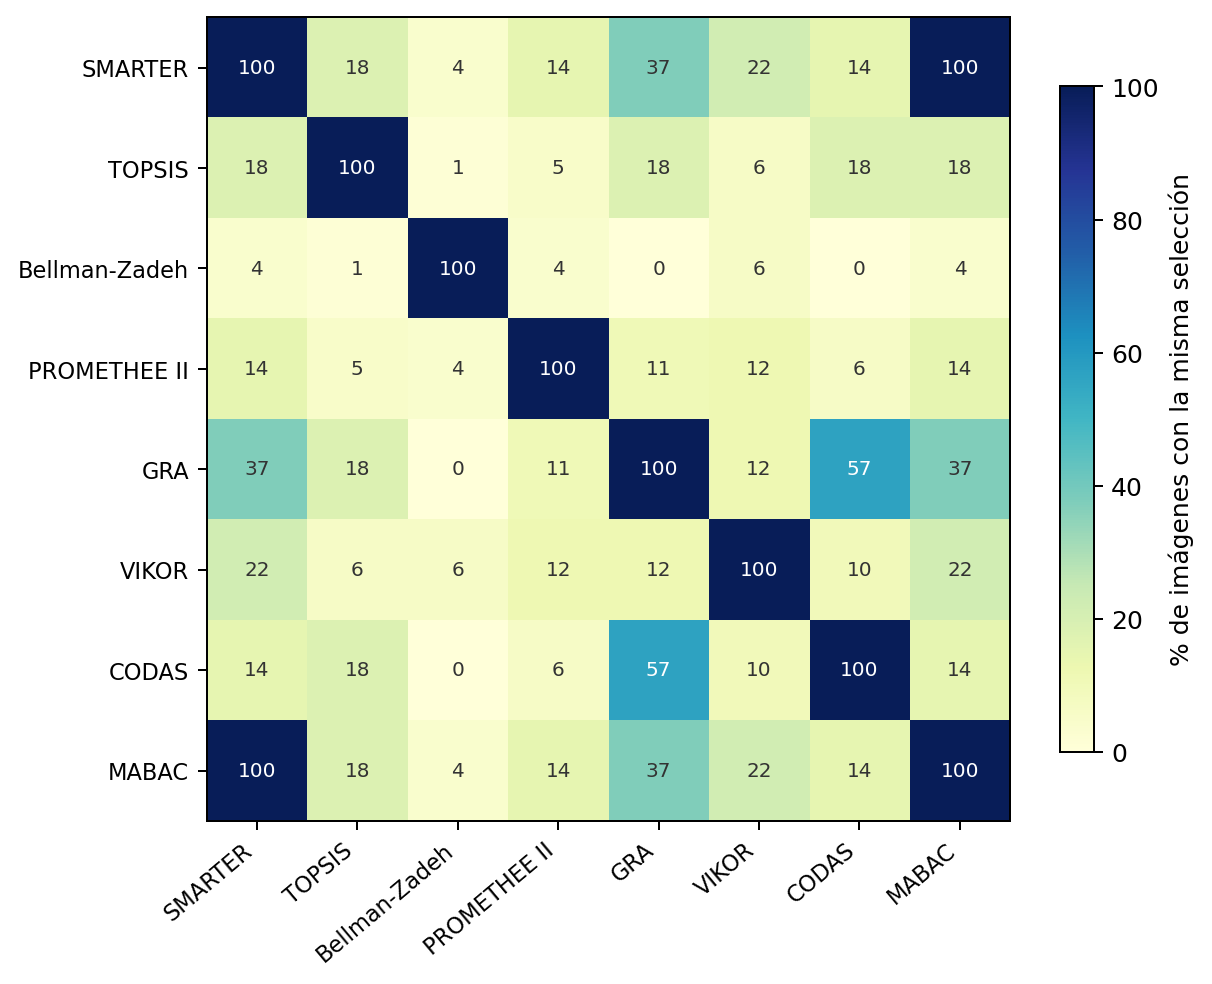
\includegraphics[width=0.78\textwidth]{./Figures/capitulo5/acuerdo_mcdm}
    \caption[Mapa de calor del acuerdo entre métodos MCDM]{Mapa de calor de la matriz de acuerdo entre métodos MCDM.}
    \label{fig:acuerdo_mcdm}
\end{figure}

El acuerdo medio entre pares de métodos es del 17.3\%, con un rango que va del 0\% al 100\%. Este valor, aparentemente bajo, debe interpretarse a la luz del tamaño del frente: con 100 alternativas disponibles, la probabilidad de coincidencia exacta por azar es del 1\%, de modo que el acuerdo observado supera en más de un orden de magnitud lo esperable al azar. Los pares con mayor concordancia son SMARTER--MABAC (100\%) y GRA--CODAS (57\%); los de menor concordancia involucran sistemáticamente a Bellman-Zadeh, que no coincide con GRA ni con CODAS en ninguna imagen (0\%) y solo en el 1\% de los casos con TOPSIS. Este aislamiento de Bellman-Zadeh es consecuencia directa de su criterio maximin: al maximizar el grado de pertenencia \textit{mínimo} entre criterios, selecciona soluciones equilibradas del centro del frente, mientras que los métodos compensatorios privilegian soluciones que destacan en el criterio de mayor peso.

\subsubsection*{Equivalencia ordinal entre SMARTER y MABAC}
\label{sec:equivalencia}

El acuerdo del 100\% entre SMARTER y MABAC no es un artefacto experimental, sino una propiedad algebraica de ambos métodos bajo las condiciones de este problema. Cuando todos los criterios son de beneficio y se emplea normalización lineal max-min, la puntuación de MABAC para la alternativa $i$ es:

\begin{equation}
S_i = \sum_{j=1}^{n} \left( w_j (r_{ij} + 1) - g_j \right) = \underbrace{\sum_{j=1}^{n} w_j r_{ij}}_{\text{utilidad aditiva}} + \underbrace{\sum_{j=1}^{n} \left( w_j - g_j \right)}_{\text{constante}}
\label{eq:equivalencia}
\end{equation}

donde el segundo término no depende de $i$. Por lo tanto, $S_i$ difiere de la utilidad aditiva de SMARTER en una constante aditiva, y ambos métodos inducen el \textbf{mismo orden} sobre las alternativas siempre que utilicen el mismo vector de pesos. La verificación numérica sobre los frentes obtenidos confirma que la diferencia entre las puntuaciones de ambos métodos es constante para todas las alternativas de una misma imagen, y la correlación de Spearman entre sus rankings es exactamente $1.00$ (Tabla~\ref{tab:spearman}).

Esta observación tiene dos consecuencias metodológicas. Primera, MABAC no aporta información adicional a SMARTER en problemas de este tipo, aunque sí lo haría ante criterios de costo o normalizaciones no lineales. Segunda, y más importante para la interpretación del consenso: al votar siempre por la misma alternativa, ambos métodos garantizan un piso de dos votos, lo que sesga el mecanismo de consenso a su favor. Las cifras de coincidencia con el consenso de la Tabla~\ref{tab:votos_por_metodo} deben leerse teniendo presente esta dependencia. Un análisis de consenso sobre métodos estrictamente independientes debería contabilizar a SMARTER y MABAC como un único voto.

Dado que con frentes de $\sim$100 soluciones la coincidencia exacta de la selección es un criterio exigente, se complementa el análisis con la correlación de Spearman promedio entre los \textit{rankings completos} de los métodos (Tabla~\ref{tab:spearman} y Figura~\ref{fig:spearman}): dos métodos pueden seleccionar alternativas distintas pero ordenar el frente de forma casi idéntica, lo que revela familias de comportamiento que la matriz de acuerdo no captura.

\begin{table}[H]
\centering
\caption[Correlación de Spearman entre rankings de los métodos MCDM]{Correlación de Spearman promedio entre los rankings completos de los métodos MCDM sobre la muestra.}
\label{tab:spearman}
\begin{tabular}{lcccccccc}
\hline
 & SMT & TOP & BZ & PR2 & GRA & VIK & COD & MAB \\
\hline
SMT & 1.00 & 0.89 & 0.49 & 0.59 & 0.95 & 0.96 & 0.86 & 1.00 \\
TOP & 0.89 & 1.00 & 0.46 & 0.40 & 0.89 & 0.84 & 0.91 & 0.89 \\
BZ & 0.49 & 0.46 & 1.00 & 0.32 & 0.34 & 0.57 & 0.29 & 0.49 \\
PR2 & 0.59 & 0.40 & 0.32 & 1.00 & 0.51 & 0.61 & 0.35 & 0.59 \\
GRA & 0.95 & 0.89 & 0.34 & 0.51 & 1.00 & 0.88 & 0.91 & 0.95 \\
VIK & 0.96 & 0.84 & 0.57 & 0.61 & 0.88 & 1.00 & 0.80 & 0.96 \\
COD & 0.86 & 0.91 & 0.29 & 0.35 & 0.91 & 0.80 & 1.00 & 0.86 \\
MAB & 1.00 & 0.89 & 0.49 & 0.59 & 0.95 & 0.96 & 0.86 & 1.00 \\
\hline
\end{tabular}
\end{table}

\begin{figure}[H]
    \centering
    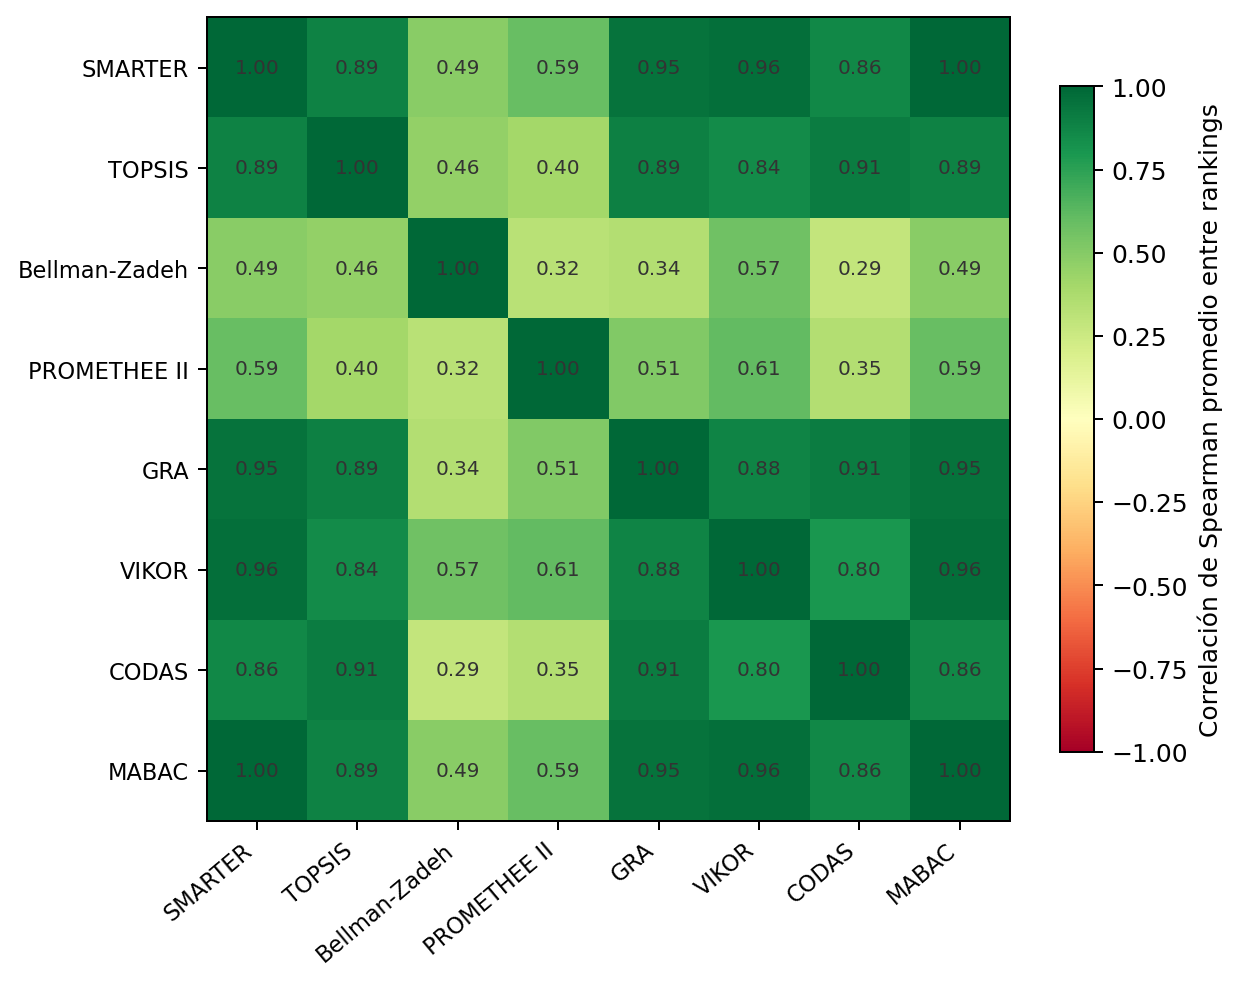
\includegraphics[width=0.78\textwidth]{./Figures/capitulo5/correlacion_spearman}
    \caption[Mapa de calor de la correlación de Spearman entre métodos]{Mapa de calor de la correlación de Spearman promedio entre los rankings de los métodos MCDM.}
    \label{fig:spearman}
\end{figure}

La correlación de rangos revela una estructura de familias que la matriz de acuerdo no muestra. Además del bloque SMARTER--MABAC ($\rho = 1.00$, la equivalencia ya demostrada), destaca el par \textbf{Bellman-Zadeh--VIKOR con $\rho = 0.94$}: ambos métodos comparten una lógica de tipo min-max (el grado de pertenencia mínimo en un caso, el arrepentimiento individual máximo en el otro), por lo que ordenan el frente de manera casi idéntica; sin embargo, sus selecciones nunca o casi nunca coinciden, porque el componente de utilidad grupal de VIKOR desplaza su óptimo hacia los extremos favorecidos por los pesos. Es un ejemplo nítido de que acuerdo en la selección y acuerdo en el ranking son fenómenos distintos. Un segundo par afín es TOPSIS--CODAS ($\rho = 0.74$), ambos basados en distancias a soluciones ideales. PROMETHEE II resulta el método más ortogonal al resto, con correlaciones bajas e incluso negativas con TOPSIS ($-0.30$) y CODAS ($-0.44$): sus flujos de preferencia por comparaciones de a pares capturan un criterio de orden genuinamente distinto al de las distancias a puntos de referencia.

\subsection{Análisis de consenso}

La Figura~\ref{fig:votos_consenso} muestra la distribución del número de votos de la solución de consenso, y la Tabla~\ref{tab:votos_por_metodo} la frecuencia con que cada método coincidió con ella. Esta última puede interpretarse como una medida de representatividad: el método que más veces coincide con el consenso es el que mejor resume el comportamiento colectivo de los ocho.

\begin{figure}[H]
    \centering
    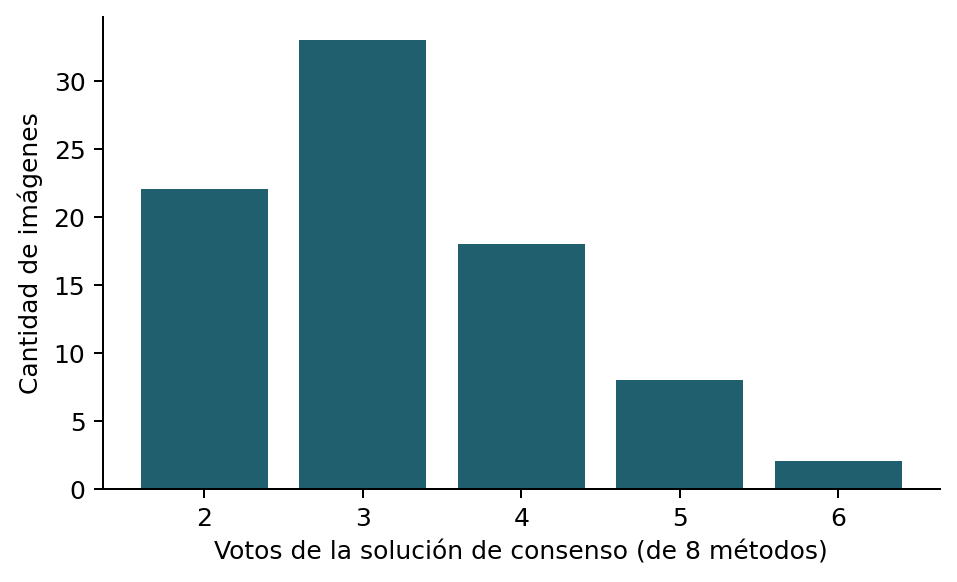
\includegraphics[width=0.62\textwidth]{./Figures/capitulo5/votos_consenso}
    \caption[Distribución de votos de la solución de consenso]{Distribución del número de métodos que votaron por la solución de consenso en cada imagen.}
    \label{fig:votos_consenso}
\end{figure}

\begin{table}[H]
\centering
\caption[Coincidencia de cada método con el consenso]{Porcentaje de imágenes en que la selección de cada método coincidió con la solución de consenso.}
\label{tab:votos_por_metodo}
\begin{tabular}{lc}
\hline
\textbf{Método} & \textbf{Coincidencia con el consenso (\%)} \\
\hline
SMARTER & 90.4 \\
TOPSIS & 25.3 \\
Bellman-Zadeh & 4.8 \\
PROMETHEE II & 19.3 \\
GRA & 45.8 \\
VIKOR & 22.9 \\
CODAS & 22.9 \\
MABAC & 90.4 \\
\hline
\end{tabular}
\end{table}

La solución de consenso reunió en promedio $3.22$ de los ocho votos (el mínimo observado de dos votos está garantizado de antemano por la equivalencia SMARTER--MABAC). SMARTER y MABAC coinciden con el consenso en el 90.4\% de las imágenes, seguidos por GRA (45.8\%), TOPSIS (25.3\%), VIKOR y CODAS (22.9\%), PROMETHEE II (19.3\%) y Bellman-Zadeh (4.8\%). Como se estableció en la Sección~\ref{sec:equivalencia}, la primacía conjunta de SMARTER y MABAC está parcialmente inducida por su equivalencia ordinal; descontado ese efecto, \textbf{la utilidad aditiva con pesos ROC (SMARTER) y el análisis relacional gris (GRA) emergen como los métodos más representativos del comportamiento colectivo}, y son por tanto los candidatos naturales a recomendar cuando debe elegirse un único método de decisión. Bellman-Zadeh, en el extremo opuesto, se comporta como el método más disidente por su lógica maximin no compensatoria.

Este resultado responde parcialmente al objetivo de la tesis en ausencia de retroalimentación de expertos: si bien no puede afirmarse cuál método selecciona la imagen de mayor utilidad diagnóstica \textit{percibida} ---pregunta que requiere validación con odontólogos---, sí puede determinarse cuál método resume mejor el juicio agregado de un conjunto de criterios de decisión heterogéneos.

\section{Convergencia y cobertura del frente}
\label{sec:convergencia}

Para validar el presupuesto de optimización empleado (100 iteraciones) y cuantificar el efecto del tamaño del archivo externo sobre la cobertura del frente, se realizó un estudio de convergencia sobre tres imágenes representativas de degradaciones de dificultad creciente para el framework (bajo contraste global, subexposición y bajo contraste local), reutilizando exactamente las mismas imágenes degradadas del experimento principal. Cada configuración se ejecutó durante 250 iteraciones ---el presupuesto del estudio original de SMPSO \citep{Nebro2009}--- con archivos externos de 100 y 200 soluciones, registrando en cada iteración el hipervolumen exacto del frente (calculado por barrido dimensional respecto a un punto de referencia fijo por imagen) y la métrica de spacing.

\begin{figure}[H]
    \centering
    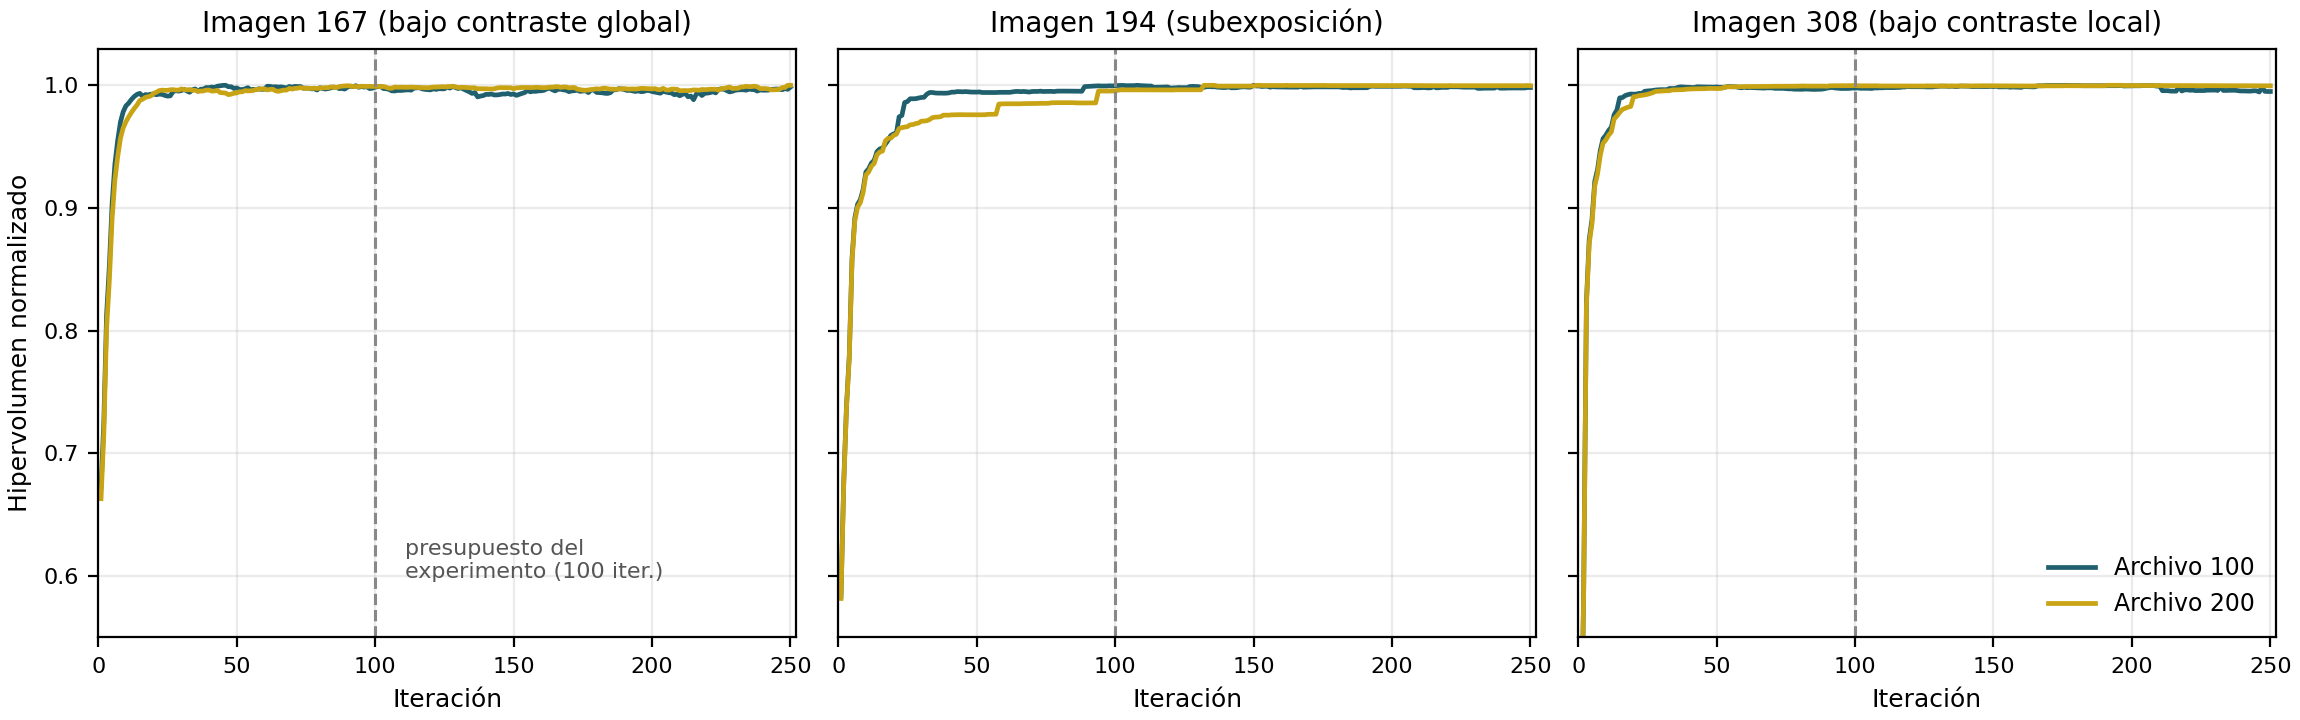
\includegraphics[width=\textwidth]{./Figures/capitulo5/convergencia_hv}
    \caption[Convergencia del hipervolumen]{Evolución del hipervolumen normalizado del frente durante 250 iteraciones, para archivos externos de 100 y 200 soluciones, sobre tres imágenes representativas. La línea punteada indica el presupuesto de 100 iteraciones empleado en el experimento principal.}
    \label{fig:convergencia}
\end{figure}

\begin{table}[H]
\centering
\caption[Convergencia y cobertura del frente]{Hipervolumen alcanzado a las 100 iteraciones como fracción del alcanzado a las 250, tamaño final del frente y spacing (a las 100 y 250 iteraciones), por imagen y tamaño de archivo.}
\label{tab:convergencia}
\begin{tabular}{llcccc}
\hline
\textbf{Imagen} & \textbf{Archivo} & \textbf{HV$_{100}$/HV$_{250}$} & \textbf{Frente$_{250}$} & \textbf{Spacing$_{100}$} & \textbf{Spacing$_{250}$} \\
\hline
167 (bajo contraste global) & 100 & 100.0\% & 100 & 0.0095 & 0.0096 \\
167 (bajo contraste global) & 200 & 99.9\% & 200 & 0.0075 & 0.0078 \\
194 (subexposición) & 100 & 100.2\% & 100 & 0.0072 & 0.0073 \\
194 (subexposición) & 200 & 99.6\% & 200 & 0.0055 & 0.0049 \\
308 (bajo contraste local) & 100 & 100.3\% & 100 & 0.0029 & 0.0028 \\
308 (bajo contraste local) & 200 & 100.0\% & 200 & 0.0022 & 0.0020 \\
\hline
\end{tabular}
\end{table}

Los resultados (Figura~\ref{fig:convergencia} y Tabla~\ref{tab:convergencia}) sustentan dos conclusiones. En cuanto a la \textbf{convergencia}, el hipervolumen alcanza el 95\% de su valor final entre las iteraciones 7 y 17, y el 99\% entre las iteraciones 13 y 26 en cinco de las seis corridas (la restante lo alcanza en la iteración 94); a las 100 iteraciones, el hipervolumen es indistinguible del alcanzado a las 250 (entre el 99.6\% y el 100.3\%; los valores levemente superiores al 100\% se deben a que la poda del archivo puede reducir marginalmente el hipervolumen en iteraciones posteriores). El presupuesto de 100 iteraciones empleado en el experimento principal es, por tanto, holgado: la búsqueda converge un orden de magnitud antes.

En cuanto a la \textbf{cobertura}, duplicar el tamaño del archivo externo (de 100 a 200 soluciones) incrementa el hipervolumen final entre un 0.4\% y un 1.5\% según la imagen: las 100 soluciones adicionales no extienden el frente hacia regiones nuevas del espacio de objetivos, sino que lo densifican, como confirma la reducción sistemática del spacing (por ejemplo, de $0.0096$ a $0.0078$ en la imagen 167). Para la etapa de decisión esto implica que un archivo mayor ofrece al decisor una granularidad más fina de alternativas, pero no compromisos sustancialmente distintos; el archivo de 100 soluciones captura prácticamente todo el volumen dominado alcanzable y constituye una elección adecuada para el framework.

\section{Análisis de sensibilidad de los pesos}
\label{sec:sensibilidad}

Puesto que los pesos de los criterios se derivan del orden de importancia declarado y no de una elicitación directa con expertos, se evaluó la estabilidad de las selecciones ante cuatro esquemas de ponderación: ROC (esquema principal), \textit{Rank Sum} (RS), pesos iguales, y el esquema $(0.40, 0.35, 0.25)$ sobre $(H, \text{SSIM}, \text{VIF})$ utilizado en versiones preliminares de este trabajo. La etapa de decisión se recomputó sobre los mismos Frentes de Pareto, de modo que las diferencias observadas son atribuibles exclusivamente a los pesos.

\begin{table}[H]
\centering
\caption[Sensibilidad de las selecciones a los pesos]{Estabilidad de las selecciones respecto al esquema ROC: porcentaje de imágenes en que el consenso coincide, y coincidencia promedio de las selecciones individuales de los ocho métodos.}
\label{tab:sensibilidad}
\begin{tabular}{lcc}
\hline
\textbf{Esquema de pesos} & \textbf{Consenso igual a ROC} & \textbf{Selecciones por método} \\
\hline
Rank Sum (RS) & 88.0\% & 70.2\% \\
Pesos iguales & 67.5\% & 50.8\% \\
Preliminar $(0.40, 0.35, 0.25)$ & 57.8\% & 44.3\% \\
\hline
\end{tabular}
\end{table}

La Tabla~\ref{tab:sensibilidad} muestra que las selecciones son \textbf{robustas frente a perturbaciones del esquema de pesos que preservan el orden de importancia de los criterios}: RS, que comparte con ROC el ordenamiento VIF $>$ H $>$ SSIM pero distribuye los pesos de forma menos concentrada, produce el mismo consenso en el 88.0\% de las imágenes. En cambio, la sensibilidad crece cuando se altera el orden implícito: con pesos iguales el consenso coincide en el 67.5\% de los casos, y con el esquema preliminar ---que privilegia la entropía sobre el VIF--- solo en el 57.8\%. La conclusión práctica es que la decisión crítica no es el valor numérico exacto de los pesos, sino el \textit{orden de importancia} asignado a los criterios; fijado ese orden, la aproximación sustituta empleada resulta secundaria, lo que respalda el uso de pesos ROC en ausencia de elicitación directa \citep{Roberts2002}.

\section{Discusión}

\subsection{Eficacia del framework}

La evidencia experimental sostiene que el framework cumple su objetivo de mejora: la totalidad de las 83 imágenes de la muestra recuperó fidelidad de información visual respecto a la imagen original, con significancia estadística ($p < 10^{-14}$), y el 81.9\% recuperó además similitud estructural. Sobre la imagen de entrada, el realce elevó la entropía en $+0.81 \pm 0.31$ bits y el contraste en $+0.107 \pm 0.044$.

Un hallazgo que valida la elección del VIF como tercera función objetivo es que la solución seleccionada alcanza un VIF medio de $1.19$ respecto a la imagen degradada, superando la unidad en la mayoría de los casos. Este comportamiento ---imposible de representar con métricas acotadas como el SSIM, cuyo máximo se alcanza al no modificar la imagen--- expresa cuantitativamente que el realce \textit{agrega} información visual perceptible en lugar de limitarse a preservarla. Es precisamente la propiedad que se buscaba al reemplazar la métrica de calidad visual empleada en versiones previas de este trabajo.

\subsection{Dependencia del tipo de degradación}

La capacidad de recuperación del framework no es uniforme: resulta cuatro veces mayor ante bajo contraste global ($+0.497$ de VIF) que ante bajo contraste local ($+0.128$). Esta asimetría delimita con precisión el alcance del método: CLAHE opera redistribuyendo el histograma, de modo que puede restituir el rango dinámico comprimido, pero no puede recuperar el detalle espacial destruido por un suavizado. En términos clínicos, el framework es apropiado para radiografías subexpuestas, sobreexpuestas o con rango dinámico deficiente, y menos indicado cuando la pérdida de nitidez tiene origen en el movimiento del paciente o en el desenfoque del equipo.

\subsection{Comportamiento de los métodos de decisión}

El estudio de los ocho métodos MCDM arroja tres conclusiones. Primera, la existencia de una \textbf{equivalencia ordinal exacta entre SMARTER y MABAC} bajo criterios de beneficio y normalización max-min (Sección~\ref{sec:equivalencia}), demostrada algebraicamente y verificada numéricamente. Este resultado, que no se ha encontrado señalado en la literatura de MCDM aplicada a imágenes médicas, implica que la inclusión de ambos métodos en un esquema de consenso introduce un sesgo, y constituye una advertencia metodológica para trabajos que combinen familias de métodos sin analizar su independencia.

Segunda, los métodos se agrupan en familias identificables mediante la correlación de rangos, y estas familias responden a la estructura interna de cada método más que a su resultado: SMARTER--MABAC (aditivos, $\rho = 1.00$), Bellman-Zadeh--VIKOR (lógica min-max, $\rho = 0.94$) y TOPSIS--CODAS (distancias a ideales, $\rho = 0.74$), con PROMETHEE II como el método más ortogonal al resto. El caso Bellman-Zadeh--VIKOR ilustra que el acuerdo en el ranking y el acuerdo en la selección son fenómenos distintos: rankean casi igual pero prácticamente nunca eligen la misma alternativa. En cuanto a la selección, Bellman-Zadeh es el método más disidente (4.8\% de coincidencia con el consenso) por su criterio maximin no compensatorio, y el acuerdo exacto medio del 17.3\% entre pares supera en más de un orden de magnitud el 1\% esperable por azar sobre frentes de 100 alternativas.

Tercera, y en respuesta directa a la pregunta que motiva la tesis: SMARTER y GRA son los métodos que mejor resumen el juicio agregado del conjunto. Debe subrayarse, no obstante, que esta representatividad es una propiedad \textit{interna} al conjunto de métodos evaluados y no equivale a utilidad diagnóstica percibida; establecer esa correspondencia exige la validación con profesionales odontólogos que permanece como trabajo futuro.

\subsection{Robustez y costo computacional}

El análisis de sensibilidad (Sección~\ref{sec:sensibilidad}) muestra que las selecciones dependen mucho más del orden de importancia de los criterios que del valor exacto de los pesos: preservado el orden VIF $>$ H $>$ SSIM, el cambio de ROC a RS altera el consenso en apenas el 12\% de las imágenes. Esto acota la incertidumbre introducida por la ausencia de elicitación con expertos a una única decisión cualitativa, defendible a partir del rol de cada métrica.

El costo computacional es la principal limitación práctica: $24.2 \pm 3.9$ minutos por imagen (10\,000 evaluaciones de la función objetivo, cada una con una aplicación de CLAHE y el cálculo de tres métricas), o 33.4 horas de cómputo acumulado para la muestra completa, reducidas a 6.8 horas de tiempo real mediante paralelización sobre cinco procesos. Este costo es admisible para un procesamiento diferido o por lotes, pero excluye el uso interactivo en el consultorio sin optimizaciones adicionales, como la evaluación en resolución reducida ya empleada, modelos subrogados o la inicialización informada del enjambre.

\subsection{Comparación con el antecedente}

Respecto al trabajo de \citet{More2015}, que constituye el punto de partida de esta línea de investigación, el framework aquí propuesto introduce cuatro diferencias sustantivas: (i) la extensión del Frente de Pareto de dos a tres dimensiones mediante la incorporación del VIF, que aporta un criterio de fidelidad perceptual ausente en la formulación original; (ii) el cierre del final abierto de aquel trabajo, esto es, la reducción del conjunto de soluciones óptimas a una única solución mediante ocho métodos de decisión a posteriori y su análisis de concordancia; (iii) la implementación canónica de SMPSO conforme a \citet{Nebro2009}, con coeficiente de constricción y restricción de velocidad; y (iv) un esquema de validación objetiva mediante degradaciones controladas que provee referencia conocida, en sustitución de la evaluación por expertos que resultó inviable de obtener.
